\documentclass[a4paper, 12pt]{article}
\usepackage[12pt]{moresize}
\usepackage[top=20mm]{geometry}
\usepackage[T1]{fontenc} 
\usepackage[utf8]{inputenc}
\usepackage{graphicx}
\usepackage[czech, english]{babel}
\selectlanguage{czech}
\usepackage{subfig}                % \subfloat
\usepackage{color}
\usepackage{url}
\usepackage{amsmath}
\inputencoding{utf8}
\usepackage{multicol}
\usepackage{caption}
\newcommand\tab[1][1cm]{\hspace*{#1}}




%--------------------------------------------------------------------------------


\begin{document}
%\maketitle
\begin{center}
	

\includegraphics[height=5cm, width=15cm]{logo}\vspace{3cm}
\LARGE{Semestrální projekt do předmětu FYO}\\\Huge{Newtonovy kroužky}
\vspace{4cm}\\ 
\LARGE{\today \\ }
\vspace{3.5cm}
\end{center}
\Large{Autor: \tab Patrik Chukir\tab <xchuki00@stud.fit.vutbr.cz>}
\normalsize
\pagebreak
\tableofcontents
\pagebreak
\section{Abstrakt}
Tato práce se bude zabývat jeve známým jako Newtonovy kroužky, jde o zvláštní případ interference na tenké vrstvě, v přírodě může být pozorován například na bublinách. V rámci textu budou popsány podmínky vzniku a chování jevu, dále jeho možná užití a nakonec popis připojené aplikace pro jednoduchou vizualizaci jevu.
\vspace{18cm}
\newline

\textbf{Klíčová slova:} Newtonovy kroužky, interference dvou vln, odraz světla 

\section{Úvod}
Při průchodu světla objektem tvořeným třemi vrstvami s tím že prostřední má různou tloušťku v různých místech vznikají obrazce odpovídající poměru tloušťky střední vrstvy a vlnové délky světla. Pokud horní materiál je tvaru kulové úseče, tedy čočky jsou tyto obrazce pravidelně kruhové a známe jako Newtonovy kroužky.
\section{Newtonovy kroužky}
 Tento jev je možno primárně pozorovat na kombinaci čočky a opticky plochého předmětu s vzduchovou mezerou krom místa dotyku, jak je možno vidět na obrázku č.\ref{cocka}.

Jev vzniká  interferencí mezi paprsky odraženými od čočky a paprsky odraženými až od podkladu. Kdy rozdíl uražených vzdáleností způsobuje fázový posun. V důsledku toho dochází v některých místech k konstruktivní/destruktivní interferenci. Pokud čočka je pravidelně kulatá výsledný obrazec je tvořen soustřednými kruhy s postupnými přechody mezi plným světlem a tmou.

To zda dojde ke konstruktivní či destruktivní interferenci je dáno rozdílem drah. Je-li tento rozdíl právě o $n\lambda$, kdy n vyjadřuje libovolné celé číslo tak potom fázový posun roven $\pi$ a dochází k destruktivní interferenci. A opačně $n\lambda + \frac{1}{2}$ dochází ke konstruktivní interferenci. Na základě tohoto jevu je možno například odvodit tloušťku vzduchové mezery. Toho se využívá u některých interferometrů.
\\

Kroužky mohou být popsány vzorcem odvozeným právě z rozdílu drah pomocí svých poloměrů.
		\begin{center}
		\begin{equation}
		\label{vzorec1}
			r_n = \sqrt{(n+\frac{1}{2}) \cdot \lambda \cdot R } 	
		\end{equation}
		\begin{equation}
		\label{vzorec2}
		r_n = \sqrt{n \cdot \lambda \cdot R } 
		\end{equation} 
		\end{center}  
 Vzorec č. 1 díky  $(n+\frac{1}{2})$ vrací poloměr n-tého světlého kroužku zatímco druhý n-tého tmavého. V obou případech počítáno od $n=0$.
  \begin{figure}
 	\begin{center}
 		
 		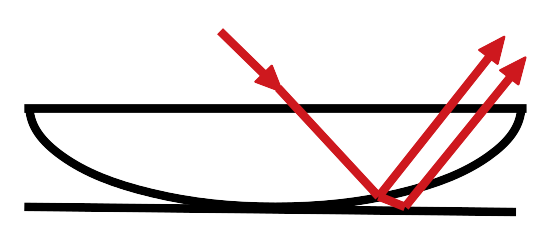
\includegraphics[width=8cm]{inter}
 		\caption{Paprsek odrážející se od čočky a podkladu }
 		\label{cocka}
 	\end{center}
 \end{figure}
  \begin{figure}

	\begin{center}
		
		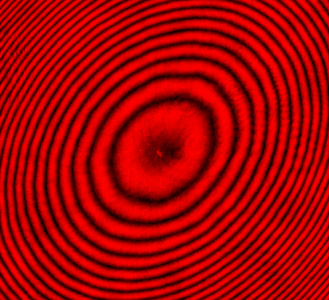
\includegraphics[width=8cm]{nr2}
		\caption{Newtonovy kroužky vzniklé 650nm laserem\cite{ceska}}
		\label{obr2}
	\end{center}
\end{figure}
\section{Původ pojmenování}
Pojmenování jevu je odvoze samozřejmě od Isaac Newton, který ten jev v 17. století využíval k porovnání kvality čoček, jejichž pomocí sestavoval teleskop. Následně tento jev popsal v publikaci kterou vydal roku 1717.

Ovšem nebyl první, kdo se tímto jeve zabýval, první jej popsal Robert Hook v roce 1664 v knize Micrographia. Ale až Isaac tento jev podrobněji zpracoval.

\section{Aplikace}
V rámci semestrální práce byla i naprogramována aplikace pro vizualizaci tohoto jevu, opravdu se jedná o pouhou vizualizaci nikoliv simulaci. Pro simulaci by musel být využit algoritmus \textit{Raycasting} nebo jemu podobný. 

Aplikace je naprogramována v C++ za pomoci NanoGui\cite{nanogui}, což jest nástavbová knihovna nad OpenGL pro grafické rozhraní. Dále v jako výchozí kostra GitHub repositáře byl použit projet NanoGui-test\cite{nanoguitest}. Aplikace umožňuje pracovat až se třemi zdroji záření a nastavit rozměry čočky(poloměr čočky a poloměr zakřivení). Nastavitelné aspekty čočky byly zvoleny dle zadání v řešených příkladech v přednáškách.
  \begin{figure}
	\begin{center}
		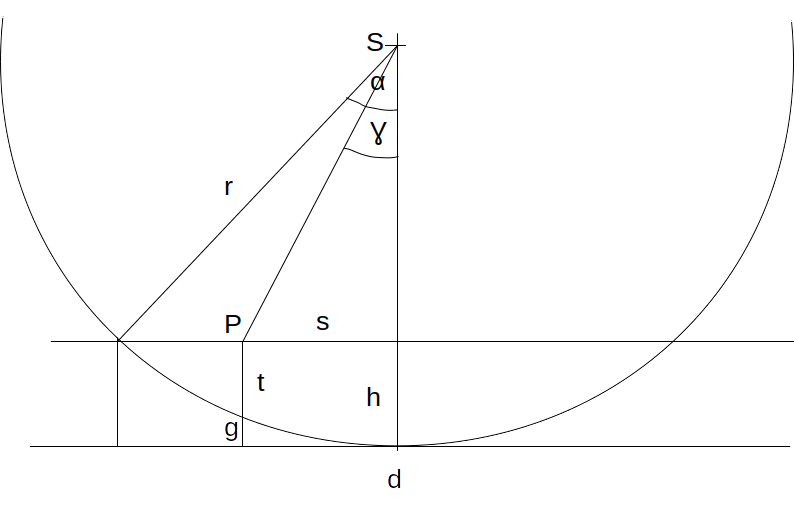
\includegraphics[width=8cm]{len}
		\caption{Náčrtek čočky}
		\label{len}
	\end{center}
\end{figure}
Výpočet probíhá per pixel. Pro každý pixel se spočítá vzdálenost od středu čočky(\ref{s}), následně úhel od osy čočky(\ref{gama}).   
		\begin{center}
	\begin{equation}
	\label{s}
	s = \sqrt{x^2 + y^2 } 	
	\end{equation}
	\begin{equation}
	\label{gama}
	\gamma = arctan(\frac{s \cdot d}{r-h})	
	\end{equation}
	\begin{equation}
	\label{right}
	g = r*(1 - cos(\alpha))	
	\end{equation}
\end{center} 
Dále by se měla získat tloušťka na základě vzorce \ref{right}, ale tento vzorec z nějakého důvodu rozkmitával(rozostřoval) výsledek.Pravděpodobně zvětšoval zaokrouhlovací chybu \textit{"floatů"}, tzn přidával náhodný šum. Proto byl místo něj využit vzorec \ref{use}, který dává vizuálně mnohem kvalitnější výsledky,ale není matematicky odvozen. Nakonec je výsledná barva pixelu spočítaná dle vzorce č. \ref{gama2} a \ref{right2}
		\begin{center}
	\begin{equation}
	\label{use}
	g = h \cdot (1 - cos(\gamma \cdot \frac{\pi}{\alpha}))  	
	\end{equation}
	\begin{equation}
	\label{gama2}
	intesity = \frac{2 \cdot g}{\lambda \cdot 0.5}
	\end{equation}
	\begin{equation}
	\label{right2}
	color = LightColor \cdot intesity	
	\end{equation}
\end{center} 

Jak je vidět na obrázcích \ref{sc1} až \ref{sc3} v Aplikaci je možno vizualizovat jev vzniklí pomocí až třech koherentních monochromatických zdrojů na čočce s definovaným poloměrem zakřivením. Přesnost výpočtu je přímo ovlivněna velikostí okna, neboť samotný výpočet probíhá ve \textit{fragment shaderu}, tedy per pixel.
  \begin{figure}
	\begin{center}
		
		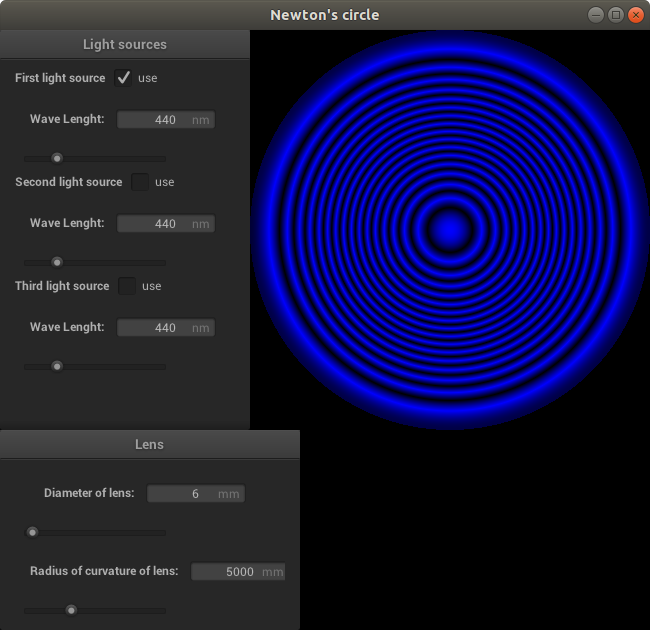
\includegraphics[width=8cm]{sc1}
		\caption{Screenshot vizualizace aplikace  při vlnové délce 440 nm }
		\label{sc1}
	\end{center}
\end{figure}
  \begin{figure}
	\begin{center}
		
		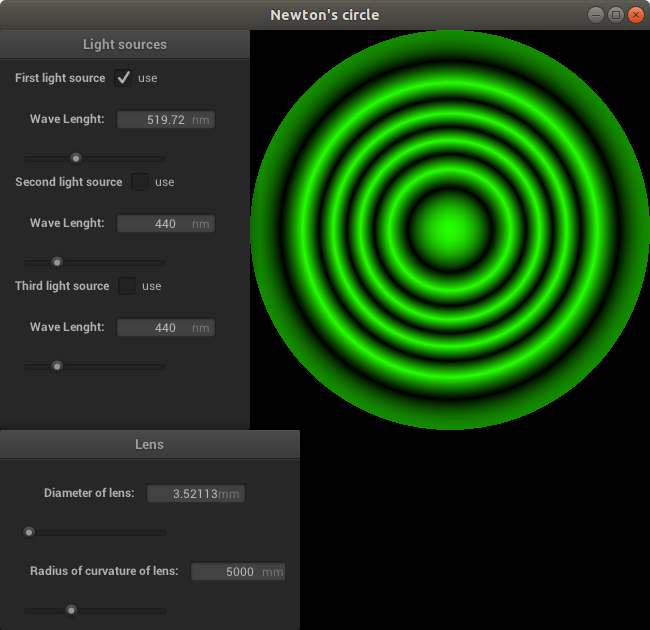
\includegraphics[width=8cm]{sc2}
		\caption{Screenshot vizualizace aplikace  při vlnové délce 519.72 nm}
		\label{sc2}
	\end{center}
\end{figure}
  \begin{figure}
	\begin{center}
		
		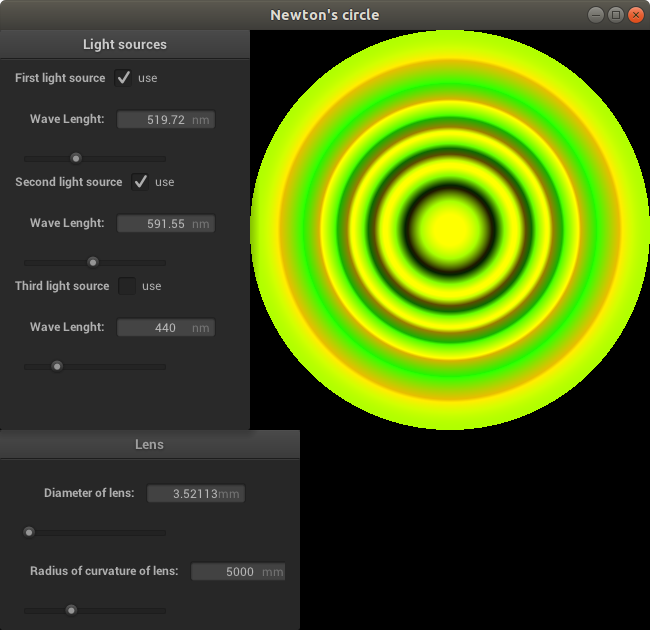
\includegraphics[width=8cm]{sc3}
		\caption{Screenshot vizualizace aplikace  při vlnové délce 519.72 nm a 591.55nm}
		\label{sc3}
	\end{center}
\end{figure}
  \begin{figure}
	\begin{center}
		
		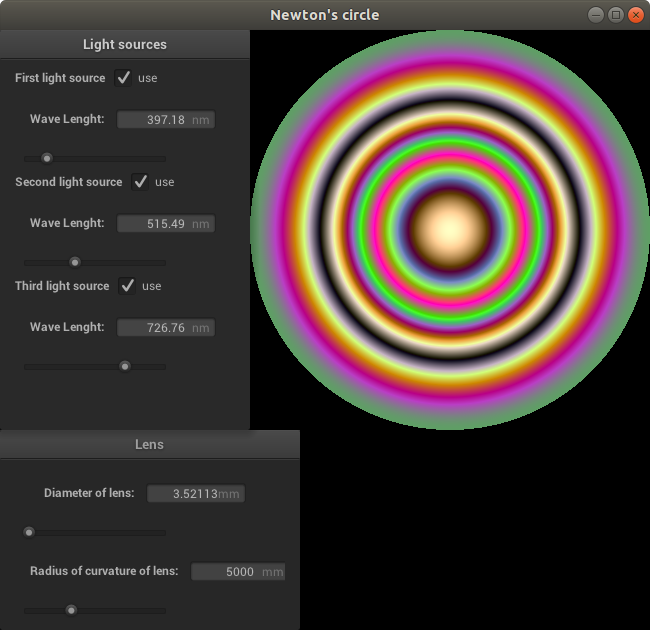
\includegraphics[width=8cm]{sc4}
		\caption{Screenshot vizualizace aplikace  při vlnové délce 397.18 nm, 515.49 nm a 726.76nm}
		\label{sc4}
	\end{center}
\end{figure}
\pagebreak
\section{Zdroje}
\begin{thebibliography}{zdroj}
	\bibitem{wiki} Wikipedie:
	\emph{Newton's Rings}. (leden 2018).\\
	\verb|https://en.wikipedia.org/wiki/Newton's_rings|
	\bibitem{homesim} Wali Khan:
	\emph{Newton's Rings}. (červen 2011).\\
	\verb|http://physical-optics.blogspot.cz/2011/06/newtons-rings.html|
	
	\bibitem{nanogui} Wenzel Jakob:
	\emph{NanoGui}. (6.3 2019).\\
	\verb|https://github.com/wjakob/nanogui|
	
	\bibitem{nanoguitest} Wali Khan:
	\emph{Newton's Rings}. (červen 2011).\\
	\verb|http://physical-optics.blogspot.cz/2011/06/newtons-rings.html|
\end{thebibliography}


\end{document}